\documentclass[10pt,a4paper,oneside,titlepage]{report}
\usepackage[utf8]{inputenc}
\usepackage[english,russian]{babel}
\usepackage{amsmath}
\usepackage{amsthm}
\usepackage{amssymb}
\usepackage{cmll}
\usepackage{enumerate}
\usepackage{stmaryrd}
\usepackage[left=2cm,right=2cm,top=2cm,bottom=2cm,bindingoffset=0cm]{geometry}
\usepackage{url}
\usepackage{listingsutf8}
\usepackage{graphicx}
\graphicspath{{pictures/}}
\DeclareGraphicsExtensions{.pdf,.png,.jpg}

\lstset{%
	numbers = left
}

\title{Конспект по курсу Машинное обучение \thanks{Читаемый Андреем Фильченковым в 2019-2020 годах}}
\author{Александра Лисицына \thanks{Студентка группы М3435}}

\theoremstyle{defenition}
\newtheorem*{defenition}{Определение}

\theoremstyle{theorem}
\newtheorem*{theorem}{Теорема}

\begin{document}
	
\maketitle

\tableofcontents

\clearpage	

\chapter{Введение}

\section{Концепция машинного обучения}

\subsection{Определения машинного обучения}

\begin{defenition}
	{\bfseries Машинное обучение} --- процесс, позволяющий компьютерам учиться, не будучи явно запрограммированными.
\end{defenition}

\begin{defenition}
	Компьютерная программа называется {\bfseries обучающейся} по некторому опыту $E$, в отношении некоторой задачи $T$ и некоторой меры производительности $P$, если его производительность на $T$, измеренная по $P$, улчшается с опытом $E$.
\end{defenition}

\begin{figure}[h!]
	\centering
	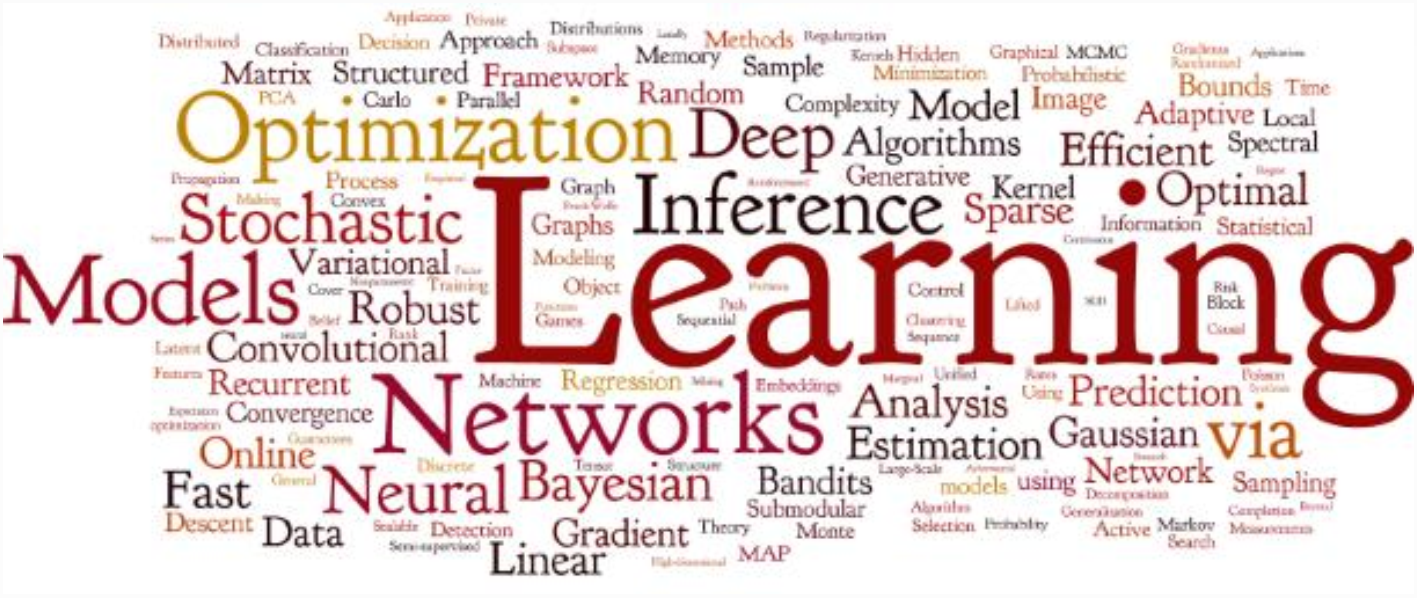
\includegraphics[width=0.7\linewidth]{pictures/MLApproaches}
	\caption{Подходы машинного обучения}
	\label{fig:mlapproaches}
\end{figure}

\begin{figure}[h!]
	\centering
	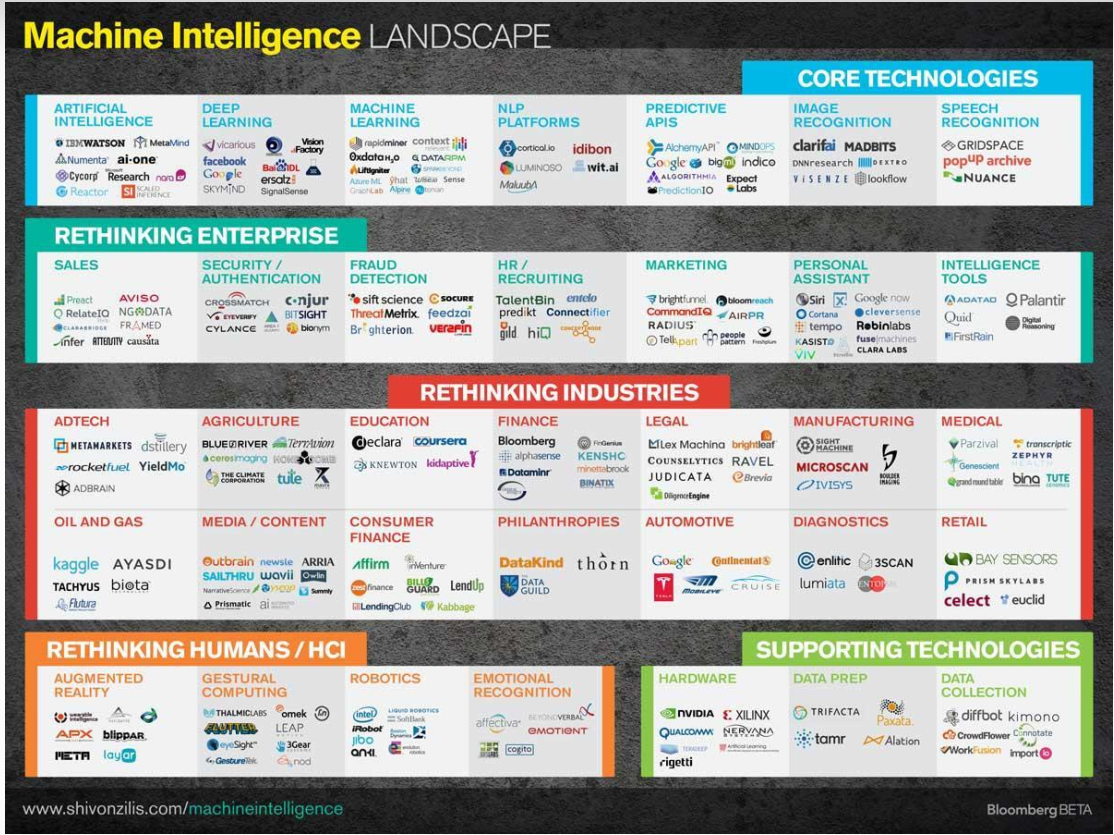
\includegraphics[width=0.7\linewidth]{pictures/MLApplications}
	\caption{Приложения машинного обучения}
	\label{fig:mlapplications}
\end{figure}

\begin{figure}[h!]
	\centering
	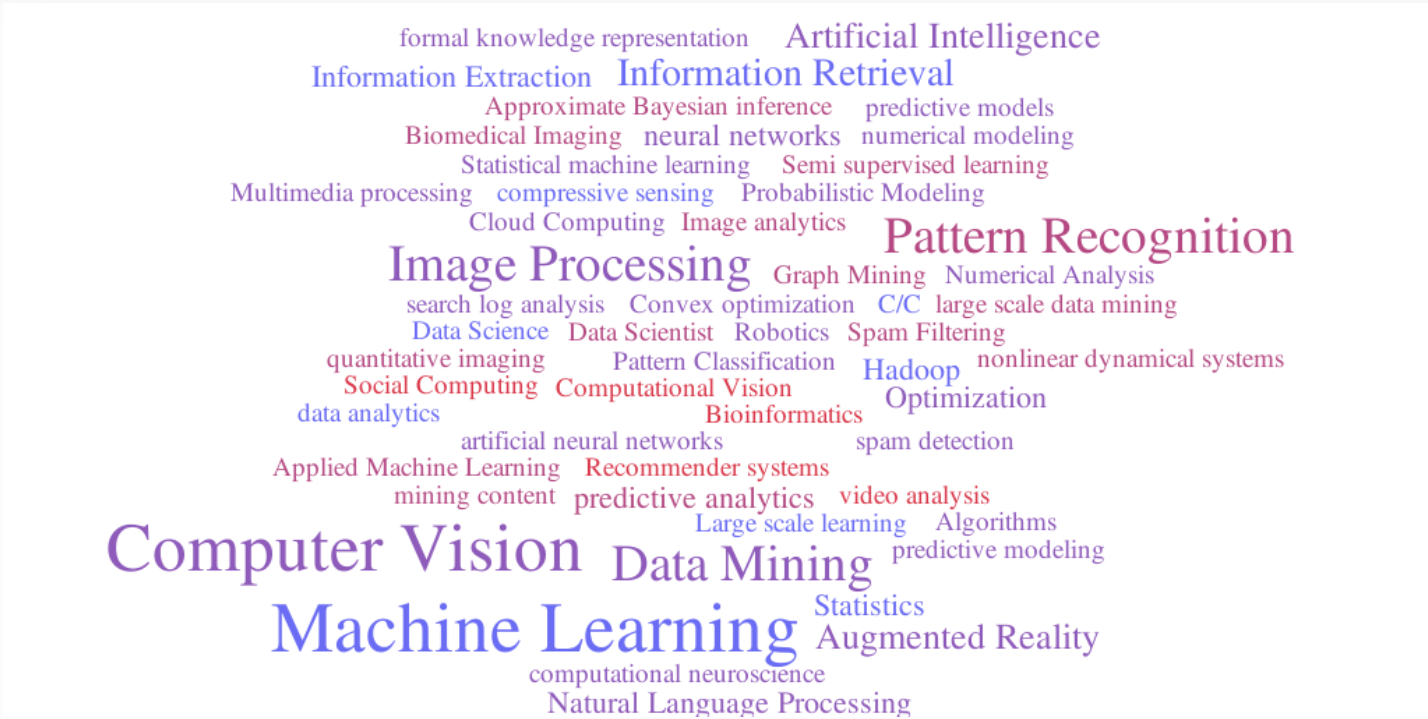
\includegraphics[width=0.7\linewidth]{pictures/RelatedConcepts}
	\caption{Родственные коцепции}
	\label{fig:relatedconcepts}
\end{figure}

\subsection{Родственные пространства}
\begin{itemize}
	\item Распознавание паттернов
	\item Компьютерное зрение
	\item Information Retrieval (IR)
	\item Natural Language Proccessing (NLP)
	\item Big Data
	\item Data Mining (Интелектуальный анализ данных)
\end{itemize}

\subsubsection{Машинное обучения vs Интелектуальный анализ данных}

Формально, интелектуальный анализ данных --- шаг в открытии знаний в базах данных. Обычно эти два термина используются как синонимы.

\begin{enumerate}
	\item Сбор данных
	\item Инженерные особенности
	\item Применение алгоритмов машинного обучения
\end{enumerate}

\subsubsection{Машинное обучение vs Наука о данных}

\begin{enumerate}
	\item Сбор данных
	\item Объединение данных
	\item Сохранение данных
	\item Анализ данных
	\item Высоко производительные вычисления
\end{enumerate}

\subsubsection{Машинное обучение vs Анализ данных}

Также известное как бизнес-аналитика

\begin{enumerate}
	\item Исследовательский анализ данных
	\item Подтверждающий анализ данных (статическая проверка гипотезы)
	\item Прогностический анализ данных
	\item Визуализация данных
\end{enumerate}

\subsection{Родственные сферы}

\begin{itemize}
	\item Искусственный интелект
	Сильный AI против слабого
	\item Интелектуальные системы
	Экспертные системы против ML систем
	\item Математическое моделирование
	\item Способы использования и представления знаний
\end{itemize}

\subsubsection{Искусственный интелект}

\begin{itemize}
	\item Сейчас у людей есть тенденция говрить AI обо всем, что родственно машинному обучению
	\item Машинное обучение --- общая часть искусственного интелекта
	\item Общий искусственный интелект (раньше сильный AI) --- более общая концепция, имеющая отношение к попытке достигнуть или превозмочь ментальные возможности человека
\end{itemize}

\subsubsection{Знания vs данные}

Знания $ne$ данные

\begin{defenition}
	{\bfseries Знания} --- это паттерны в определенной области знаний (принципы, регулярность, отношения, правила, законы), получнные с практикой и профессиональным опытом, которые помогают сформулировать и решить проблемы в определнной области.
\end{defenition}

\subsection{Требуемый бэкграунд}

\begin{itemize}
	\item Теория вероятности и математическая статистика
	\item Оптимизация
	\item Вычислительная наука
	\item Линейная алгебра
	\item Дискретная математика
	\item Теория комплексных вычислений
	\item и так далее
\end{itemize}

\subsection{Задачи машинного обучения}

\begin{itemize}
	\item Контролируемое обучение

	Дано множество примеров с ответами. Правило для получаемых ответов для всех возможных примеров требует:
	\begin{itemize}
		\item классификации
		\item регрессии
		\item обучения оцениванию
		\item прогнозирование
	\end{itemize}
	\item Неконтролируемое обучение

	Дано множество примеров без ответов. Правило для нахождения ответов или периодичности требует:
	\begin{itemize}
		\item кластеризации
		\item обучения ассоциированным правилам
		\item рекомендательных систем
		\item уменьшения размеров
	\end{itemize}
	\item Полуконтролируемое обучение
	\item Обучение с подкреплением
	\item Активное обучение
	\item Онлайн обучение
	\item Структурированный прогноз
	\item Выбор и валидация модели
\end{itemize}

\section{Контрлируемое обучение}

Большую часть времени разговор будет именно о контролируемом обучении.

\begin{figure}[h!]
	\centering
	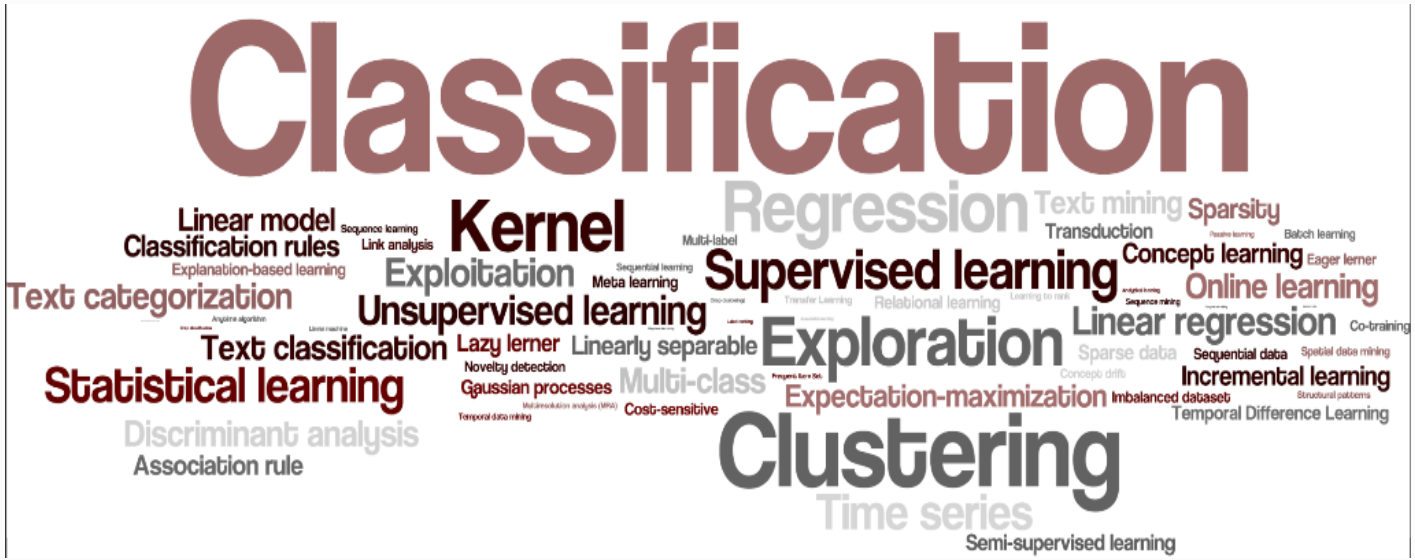
\includegraphics[width=0.7\linewidth]{pictures/SupervisedLearning}
	\caption{Контрлируемое обучени}
	\label{fig:supervisedlearning}
\end{figure}

\subsection{Задача}

$X$ --- множество объектов или входов

$Y$ --- множество меток, ответов или выходов

$y: X \to Y$ --- неизвестная целевая функция (зависимость)

$\{x_1, \dots , x_l\} \subset X$ --- тренировачное множество примеров

$y_i = y(x_i), i = 1, \dots , l$ --- известные значения функции

Задача: найти $a: X \to Y$ --- решающая функция, которая аппроксимирует $y$ на $X$.

Мы собираемся говорить только о алгоритмах.

\subsection{Главные вопросы}

\begin{enumerate}
	\item Как описаны объекты?
	\item Как выглядят объекты?
	\item Каково множество объектов, из которого мы выбираем $a$?
	\item Какова мера качества того, насколько хорошо $a$ аппроксимирует $y$?
\end{enumerate}

\subsubsection{Как описаны объекты}

$f_j: X \to D_j, j = 1, \ldots , n$ --- свойства или атрибуты

Типы свойств:
\begin{itemize}
	\item двоичный: $D_j = \{0, 1\}$
	\item категории: $D_j$ --- конечное
	\item порядковый: $D_j$ --- конечное и с порядком на элементах
	\item численный: $D_j = R$
\end{itemize}

\paragraph{Данные свойств}

$(f_1(x), \ldots , f_n(x))$ --- описание свойств объекта $x$. Объект --- это его описание свойств.

\section{Линейные методы}

\subsection{Показатели эффективности}

\subsubsection{Таблица сопряженности}

\begin{figure}[h]
	\centering
	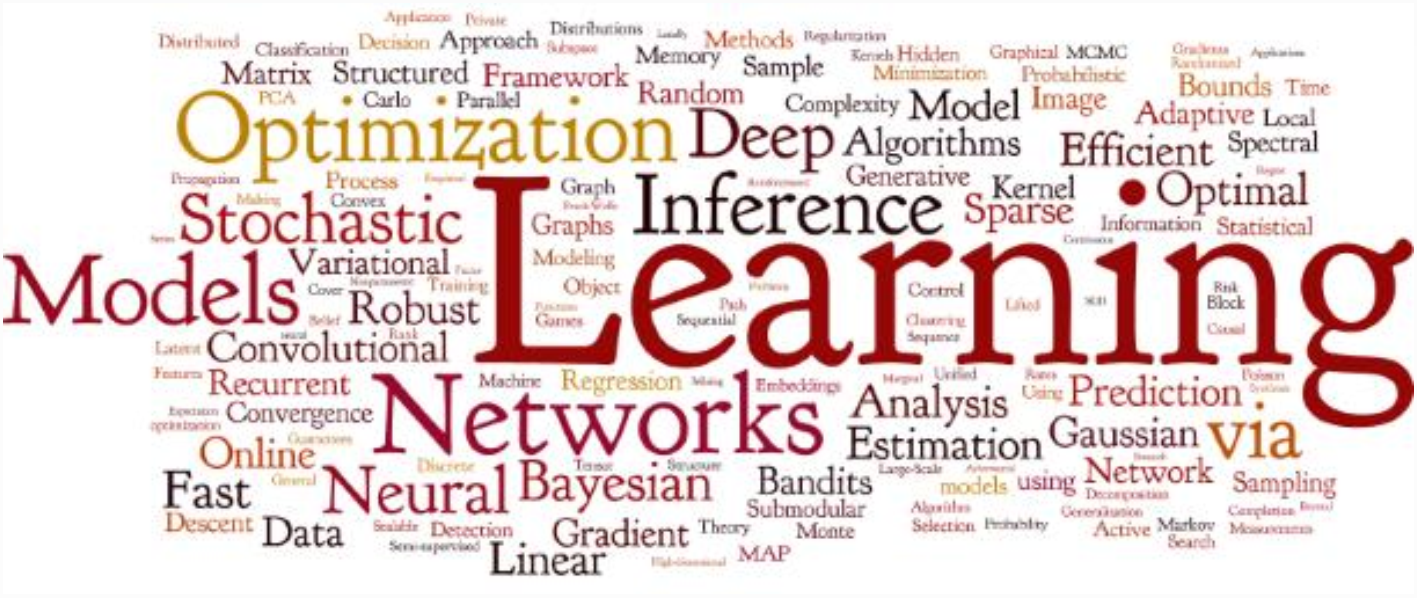
\includegraphics[width=0.7\linewidth]{pictures/screenshot001}
	\caption{Таблица сопряженности}
	\label{fig:screenshot001}
\end{figure}

В математической статистике:
\begin{itemize}
	\item FN --- ошибка первого рода
	\item FP --- ошибка второго рода
\end{itemize}

$P = TP + FN$ --- количество положительных примеров

$N = FP + TN$ --- количество негативны примеров

\subsubsection{Некоторые определения}

\begin{itemize}
	\item Полнота (Recall/Sensitivity) $Recall = TPR = \frac{TP}{P}$
	\item Specifity $SPC = \frac{TN}{N}$
	\item Точность (Precision) $Precision = PPV = \frac{TP}{TP + FP}$
	\item Точность (Accuracy) $Accuracy = ACC = \frac{TP + TN}{P + N}$
\end{itemize}

\subsubsection{F--мера}

$$
F_{\beta} = (1 + \beta^2)\cdot\frac{Precision\cdot Recall}{\beta^2\cdot Precision + Recall}
$$

\subsubsection{ROC--кривая}

\begin{defenition}
	Кривая ошибок или ROC-кривая – графичекая характеристика качества бинарного классификатора, зависимость доли верных положительных классификаций от доли ложных положительных классификаций при варьировании порога решающего правила. На графике будет не больше точек, чем объектов в обучающей выборке. По факту строится по числу различающих точки значений порога (то есть если все значения равны, будут ровно две точки). Порог решающего правила в качестве аргумента принимает любым образом выраженную степень уверенности классификатора в ответе.
\end{defenition}

%\begin{figure}[h]
%	\centering
%	\includegraphics[width=0.7\linewidth]{screenshot002}
%	\caption[ROC--кривая]{}
%	\label{fig:screenshot002}
%\end{figure}

A --- лучший алгоритм; B --- типичный; C --- худший.

\subsubsection{AUC}

\begin{defenition}
	AUC (Area Under Curve) --- площадь под ROC--кривой. Используется для численной оценки алгоритма.
\end{defenition}

\subsubsection{Случай multiclass}
Разобраться с этим случаем.
\begin{itemize}
	\item One vs One classification
	\item One vs all classification
	\item иерархическая классификация
	\item Confusion matrix
\end{itemize}

\subsubsection{Щбычные регрессионные ошибки}

\begin{itemize}
	\item Корневая средне--квадратичная ошибка (RMSE)
	\item Средняя абсолютная ошибка (MAE)
	\item Средне--квадратичная ошибка (MSE)
	\item Симметричная средняя абсолютная ошибка по процентам (SMAPE) $SMAPE = \dfrac1l \sum_{j=1}^{l}\dfrac{2\cdot |a(x_j) - y_j|}{|a(x_j)| + |y_j|}$
\end{itemize}

\subsection{Линейная классификация}

\subsubsection{Формуляция проблемы}

Ограничение: $Y = \{-1, +1\}$

$T^l = \{(x_i,y_i)\}_{i = 1}^l$ дан.

Найти классификатор $a_w(x, T^l)$ в виде $sign(f(x, w))$, где $f(x, w)$ --- функция многообразия, $w$ --- вектор параметров

Ключевая гипотеза: все объекты (хорошо) разделимы

Основан идея: искать среди раздельных поверхностей определенных с $f(x, w) = 0$

\subsubsection{Margin}

\begin{defenition}
	{\bfseries Margin} объекта $x_i$: $M_i(w) = y_if(x_i, w)$.
\end{defenition}

$M_i(w) < 0$ --- свидетельство неправильной классификации.

У нас есть предыдущее определение Margin: $M(x_i) = C_{y_i}(x_i) - max_{y\in Y\backslash\{y_i\}}$, где $C_y(u) = \sum_{i=1}^l[y(u, i) = y]w(i, u),  w(i,u)$ --- функция веса $i$го соседа $u$.

\subsubsection{Сглаживание функции потерь}

Эмпирический риск:

$$
Q(a_w, T^l) = Q(w) = \sum_i^l [M_i(w) < 0]
$$

просто количестов ошибок демонстрируемых $a_w$.

Эта функци не гладкая, поэтому трудно найти ее оптимум. 

Аппроксимация:

$$
\tilde{Q}(w) = \sum_i^l L(M_i(w)),
$$

где $L(M_i(w)) = L(a_w(x, T^l), x_i)$ --- функция потерь

Мы хотим, чтобы $L$ была неотрицательная, невозрастающая и гладкая.

\subsubsection{Линейный классификатор}

$f_j: X\rightarrow R, j = 1, \ldots, n$ --- числовые характеристики.

{\bfseries Линейный классификатор}

$$
a_w(x, T^l) = sign(\sum_{i=1}^n w_if_i(x) - w_0)
$$

$w_1, w_2, \ldots, w_n$ --- весовая характеристика.

Эквивалентная нотация:

$$
a_w(x, T^l) = sign(<w, x>)
$$

если характеристика $f_0(x) = -1$ добавлена.

\subsubsection{Нейрон}

{\bfseries McCulloch-Pitts нейрон:}

$$
a_w(x, T^l) = sigma ( \sum_{i=1}^n w_i f_i(x) - w_0)
$$

где $\sigma$ --- функция активации

\subsubsection{Множестов алгоритмов}

Это предположение о том, как следует выглядеть классификатору, специфично к множеству $A_{linear}$, из которого мы и выбираем алгоритм.

$$
A_{linear} = \{a_w(x) = sign(<w, x>) | w \in R^n\}
$$

Эмпирический риск не является blac-box функцией. И даже более того мы можем гарантировать, что она гладкая.

\subsection{Градиентный спуск}

Задача минимизации эмпирического риска:

$$
\tilde{Q}(w) = \sum_i^l L(M_i(w)) = \sum_i^l L(<w,x>y_i) \rightarrow min_w
$$

Градиентный спуск:

$w^{[0]}$ --- начальное предположение

$w^{[k+1]} = w^{[k]} - \mu\nabla Q(w^{[k]})$, где $\mu$ --- шаг градиента.

$w^{[k+1]}=w^{[k]} - \mu\sum_i^l L'(<w, x>y_i)x_iy_i$

Останавливаемся, когда значение $Q$ и/или значительно не изменяется.

\subsubsection{Min-batch градиентный спуск}

Проблема в том, что это слишком рандомно, так как зависит от единственного объекта.

$w^{[0]}$ --- начальное предположение; $b$ --- размер батча;

$x_{(1)}, x_{(2)}, \ldots, x_{(l)}$ --- объектный порядок;

$w^{[K+1]} = w^{[K]} - \mu$

\section{Probabilistic classifiers (Вероятностные классификаторы)}

\subsection{Байевская классификация}

\subsubsection{Задача}

Заболевание распространено среди 1\% популяции. Тест вовзвращает правдивый результат в 95\% случаев. Некто получил положительный результат. Какова вероятность, что он действительно болен?

\paragraph{Ответ}

$$
Pr(d = 1 | t = 1) = \frac{Pr(t = 1 | d = 1)Pr(d = 1)}{Pr(t = 1 | d = 1)Pr(d = 1) + Pr(t = 1 | d = 0)Pr(d = 0)} = \frac{0,95\cdot 0,01}{0,95\cdot0,01 + 0,05\cdot0,99} = 0,16
$$

\subsubsection{Задача вероятностной классификации}

Вместо неизвестной целовой функции $y^*(x)$, мы будем думать о неизвестном распределении на $X\times Y$ с плотностью $p(x, y)$.

\begin{defenition}
	{\bfseries Простой (независимо) одинаково распределенный пример} --- пример, состоящий из $l$ случайных независимых наблюдений $T^l = \{(x_i, y_i)\}^l_{i=1}$.
\end{defenition} 

Теперь у нас есть семейство распределений $\{\phi (x, y, \theta) | \theta \in \Theta\}$ вместо моделей алгоритма.

{\bfseries Задача:} найти алгоритм, минимизирующий вероятность ошибки.

\subsubsection{Утверждения}

$a: X\to Y$ делит $X$ на непересекающиеся области $A_y$:
$$
A_y = \{x \in X | a(x) = y\}
$$
Ошибка возникает, когда элемент $x$ с меткой $y$ классифицируется как принадлежащий $A_s, s \ne y$.

{\bfseries Вероятность ошибки:} $Pr(A_s, y) = \int_{A_s}p(x,y)dxA_s$.

{\bfseries Ошибочная потеря:} $\lambda_{sy} = \ge \forall (s, y) \in Y \times Y$.

Обычно $\lambda_{yy} = 0, \lambda_y = \lambda_{ys} = \lambda_{yt} \forall s, t \in Y, s \ne y, t \ne y$.

{\bfseries Средний риск} $a$:
$$
R(a) = \sum_{y\in Y}\sum_{s\in Y}\lambda_{ys}Pr(A_s, y)
$$ 

\subsubsection{Главное уравнение}

$$
p(X, Y) = p(x)Pr(y|x) = Pr(y)p(x|y)
$$

\begin{itemize}
	\item $Pr(y)$ --- {\bfseries априорная вероятность} класса $y$.
	\item $p(x|y)$ --- {\bfseries функция правдоподобия} класса $y$.
	\item $Pr(y|x)$ --- {\bfseries апостериорная вероятность} класса $y$.
\end{itemize}

\subsubsection{2 проблемы}

\begin{enumerate}
	\item {\bfseries Восстановление плотности вероятности:} 
	
	Дано: $T^l = \{(x_i, y_i)\}^l_{i=1}$.
	
	Задача: найти эмпирическую оценку $\hat{Pr}(y)$ и $\hat{p}(x|y), y \in Y$.
	\item {\bfseries Минимизация среднего риска:}
	
	Дано:
	\begin{itemize}
		\item априорная вероятность $Pr(y)$
		\item likelihood $p(x|y), y \in Y$
	\end{itemize}
    Задача: найти классификатор $a$, который минимизирует $R(a)$
\end{enumerate}

\subsubsection{Максимум апостериорной вероятности}

Пусть $Pr(y), p(x|y)$ известны $\forall y \in Y$
$$
p(x, y) = p(x)Pr(y|x) = Pr(y)p(x|y)
$$

{\bfseries Главная идея:} выбирать класс такой, что наблюдения принадлежеат ему с наибольшей вероятностью.

{\bfseries Максимум апостериорной вероятности (MAP): }
$$
a(x) = argmax_{y\in Y}Pr(y|x) = argmax_{y\in Y}Pr(y)p(x|y)
$$

\subsubsection{Оптимальный байесовский классификатор}

\begin{theorem}
	Если $Pr(y)$ и $p(x|y)$ известны, тогда минимальный средний риск достигается Байесовски классификатором
	$$
	a_{O}B(x) = argmin_{s\in Y}\sum_{y\in Y}\lambda_{ys}Pr(y)p(x|y)
	$$
	Если $\lambda_{yy} = 0, \lambda_y = \lambda_{ys} = \lambda_{yt} \forall s, t \in Y s \ne y, t \ne y$
	$$
	a_{OB}(x) = argmin_{y\in Y}\lambda_yPr(y)p(x|y)
	$$
	Классификатор $a_{OB}$ --- {\bfseries оптимальный Байесовский классификатор}.
	
	{\bfseries Байсовский риск} --- минимальное значение $R(a)$.
\end{theorem}

\subsubsection{Разделительная поверхность (separating surface)}

\begin{defenition}
	{\bfseries Разделительная поверхность (separating surface)} для классов $a$ и $b$ --- геометрическое местоположение точек $x \in X$, таких что максимум Байесовского правила решения достигается и для $y = a$ и $y = b$:
	$$
	\lambda_aPr(a)p(x|a) = \lambda_bPr(b)p(x|b)
	$$
\end{defenition}

\subsection{непараметрическое восстановление плотности}

\subsubsection{2 подзадачи}

Задача --- оценить априорную и апостериорную(?) вероятности для каждого класса:
$$
\hat{Pr}(y) = ?
\hat{p}(x|y) = ?
$$

Первая проблема может быть решена просто:
$$
\hat{Pr}(y) = \frac{|X_y|}{l}, X-y = \{(x_i, y_i) \in T^l, y_i = y\}
$$

Вторая проблема более сложна.

\subsubsection{Проигравший класс}

Мы можем решить:
$$
\hat{p}(x|y) = ?
$$
независимо для каждого класса.

Вместо восстановления $\hat{p}(x|y)$, мы будем восстанавливать $\hat{p}(x)$ используя $T^m = \{(x_{(1)}, s), \ldots, (x_{(m)}, s)\}, for all s \in Y$.

\subsubsection{Одномерный случай}

Если $Pr([a, b])$ вероятностная мера на $[a, b]$, тогда
$$
p(x) = \lim_{h\to0}\frac1{2h}Pr([x - h, x + h])
$$

Эмпирическая оценка плотности с окном ширины $h$:
$$
\hat{p_h}(x) = \frac1{2mh}\sum_{i=1}^m[|x - x_i| < h]
$$

\subsubsection{Окно Парзена-Розенблатта}

{\bfseries Оценка Парзена Розенблатта} для окна ширины $h$:
$$
\hat{p_h}(x) = \frac1{mh}\sum_{i=1}^mK(\frac{x - x_i}h),
$$
где $K(r)$ --- ядро.

$\hat{p_h}(x)$ сходится к $p(x)$.

\subsubsection{Обобщение для многомерного случая}

\begin{enumerate}
	\item Если объекты описаны $n$ числовыми функциями: $f_j:X \to R, j = 1, \ldots, n$
	$$
	\hat{p_h}(x) = \frac1m \sum_{i=1}^m\prod_{j=1}^n\frac1{h_j}K(\frac{f_j(x) - f_j(x_i)}{h_j}).
	$$
	\item Если $X$ метрическое пространство с расстоянием $\rho(x,x')$
	$$
	\hat{p_h}(x) = \frac1{mV(h)}\sum_{i=1}^mK(\frac{\rho(x, x_i)}h),
	$$
	где $V(h) = \int_X K(\frac{\rho(x, x_i)}h)dx$ --- коэффициент нормализации.
\end{enumerate}

\subsubsection{Многомерное окно Парзена}

Оценим $\hat{p_h}(x)$:
$$
\hat{p_h}(x) = \frac1{mV(h)}\sum_{i=1}^mK(\frac{\rho(x, x_i)}h),
$$

{\bfseries Окно Парзена:}
$$
a(x, T^k, h) = argmax_{y \in Y}\lambda_yPr(y)l_y^{-1}\sum_{i:y_i=y}K(\frac{\rho(x, x_i)}{h}),
$$
$$
\Gamma_y(x) = \lambda_yPr(y)l_y^{-1}\sum_{i:y_i=y}K(\frac{\rho(x, x_i)}{h}) \mbox{ближайший к классу}
$$

\section{Lection6}

\subsection{Логистические правила}

\subsubsection{КОнцепты и правила}

\begin{defenition}
	{\bfseries КОнцепт} --- предикат над объектом класса $X$:
	$$
	\phi
	$$
\end{defenition}

\subsubsection{интерпретируемые концепты}
Может быть итерпритируем, если:
\begin{itemize}
	\item сформулированы на естественном языке
	\item не более 7 признаков
\end{itemize}

\subsubsection{Информативные концепты}

Концепт информативен, если он может покрыть наибольшее число объектов, который нужно покрыть и наименьшее тех , которых не нужно.

\subsubsection{сигма, дельта}

\subsubsection{статистическое правило}

$$
H_{P, N}(p, n) = \frac{C_P^pC_N^n}{C_{P+N}^{p+n}}
$$
$$
I_c(\phi, T^l) = -\ln H
$$

\subsubsection{првило базирующееся на энторпии}

$$
\hat H(P, N) = H(\frac{P}{P + N}, \frac{N}{P + N})
$$
$$
$$
$$
IGain_C(\phi, T^l) = \hat H(P, N) - \hat{H_{\phi}}(P, N, p, n)
$$

\subsubsection{Дерево решений}

Дереворешений --- классификатор и регрессия.

\paragraph{Общая схема}

Придумываем множество правил и меру качества разбиения.

\begin{enumerate}
	\item Отправляем вершину в корень
	\item 
	\subitem Если вершина содержит  объекты только из одного класса, то говрим, что это лист этого класса и останавливаемся.
	\subitem Иначе выбираем разделяющее правило , наиболее точное по $\Phi$
\end{enumerate}

\subsubsection{деревья регрессии}

\chapter{Сверточные нейронные сети}

\section{Беголый взгляд на ImageNet}

\subsection{Соревнование ImageNet}

\begin{itemize}
	\item 1000 изображений в классе
	\item 1000 классов
	\item на данный момент 14 млн изображений
\end{itemize}

\section{Более ранние приближения в компьютерном зрении}

\subsection{Короткая история компьютерного зрения}

\begin{figure}[h!]
	\centering
	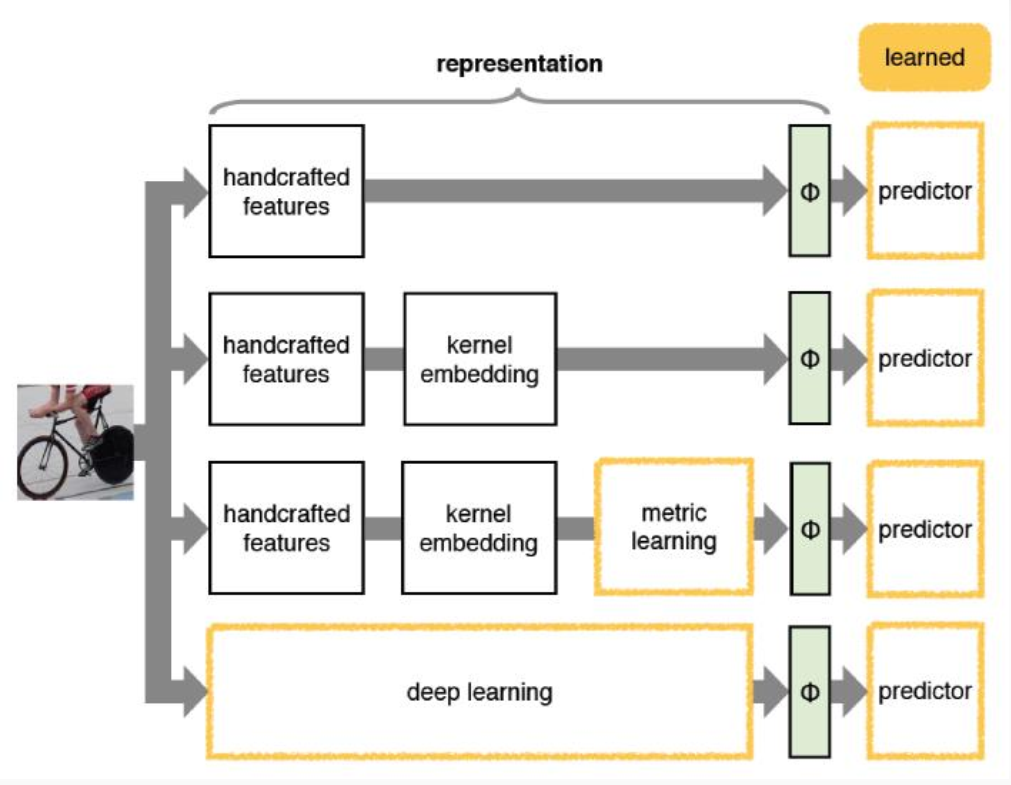
\includegraphics[width=0.4\linewidth]{pictures/ComputerVision}
	\caption{История компьютерного зрения}
	\label{fig:computervision}
\end{figure}


\section{Сверточные нейронные сети}

\section{Тензоры}

\section{Развертывание и визуализация нейронов}

\section{Обзор архитектуры}

\section{Проблемы компьютерного зрения}

\end{document}